\chapter{Results and Discussion}
\label{resultanddiscussion}


This chapter covers the results and the discussion of all tests formulated in Chapter \ref{configurationandtesting}. In addition potentially needed optimization steps will be highlighted.
\section{Odometry test}

When looking at the odometry published by the differential drive plugin during the test in Figure \ref{wheel odom} it is noticeable, that the measurement has a huge rotational error, which is expected since the wheels always slip slightly when turning a differential drive robot.
\todo{picture including true odometry}
\begin{figure}[H]
	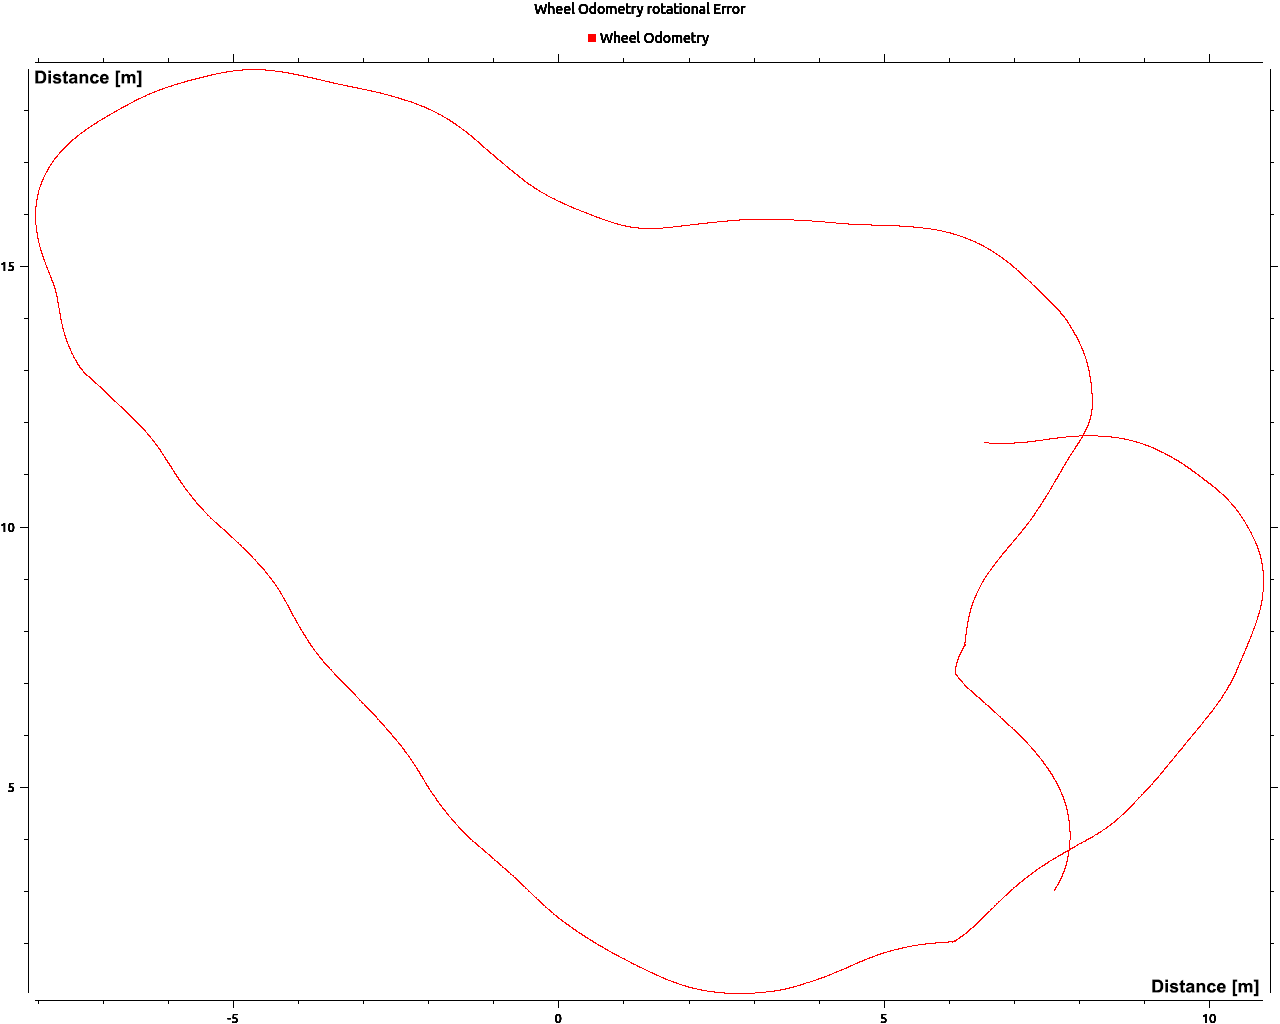
\includegraphics[width=\textwidth]{Pictures/rot error}
	\caption{Odometry Test result}
	\label{wheel odom}

\end{figure}

The quality of the odometry obviously is not sufficient and has to be improved.

\subsection{Optimization}
Since the odometry is found to not being sufficient for the navigation the following optimization approach will be tried and further testing will be performed. The test scenario will be remain the same.

To improve the odometry the ROS package robot\_localization can be used. It provides an extended kalman filter for the fusion of sensor data for odometry.\\

To reduce the rotational error, an IMU (Inertia measurement unit) will be added to the robot configuration. Both, the imu and the wheel encoder will be fused by robot\_localization.

The IMU provides the following data:
\begin{itemize}
	\item orientation
	\item angular velocity
	\item linear acceleration
\end{itemize}

In this usecase the IMU is only supposed to measure data relevant for 2D operation roll, pitch and tranlation in z (axis according to to REP 103) will not be passed to the filter. 

The IMU is used for localization purposes, therefore the linear acceleration data is not interesting, since the accelerations would need to be integrated twice to be used for the pose. This would amplify every little error in the measured acceleration and will decrease the reliability of the odometry with increasing time.\\

Accordingly the only things fused from the imu are the yaw orientation and velocity.\\

Just like the IMU data the integration of the wheel-odometry data has to be discussed which consist only from linear and angular velocities, aswell as a pose derived from the velocities.\\

Here the most interesting part is the y velocity since the robot is relying on differential drive steering and therefore not able to have instantaneous y acceleration other than drift.\\

In contrast to the acceleration values of the IMU the y velocity will be included since according to Tom Moore (the developer of robot\_localization) it will give certainty that the robot has not moved in the y direction\cite{robotlocalizationconfiguration}. Obviously the x and yaw velocity has to be included aswell.

The position component of the wheel-odometry on the other hand will not be used, based on the fact that the position is already derived from the velocitys this would include the same data twice.\\

Unfortunately this does not solve the problem of the odometry correction yet. As visible in Figure \ref{pose comparison wheel odom + IMU} the odometry of the extended kalman filter has large jumps in it compared to the wheel-odometry. When observing it in real time the ekf odometry starts to drift and jumps back after a certain amount of time.\\
Looking at the linear velocities of both the ekf and the wheel odometry in Figure \ref{velocity comparison wheel odom + IMU} it is noticeable that the ekf filter does estimate a continuous acceleration, whereas the velocity of the wheel encoders actually decreases.\\



\begin{figure}
	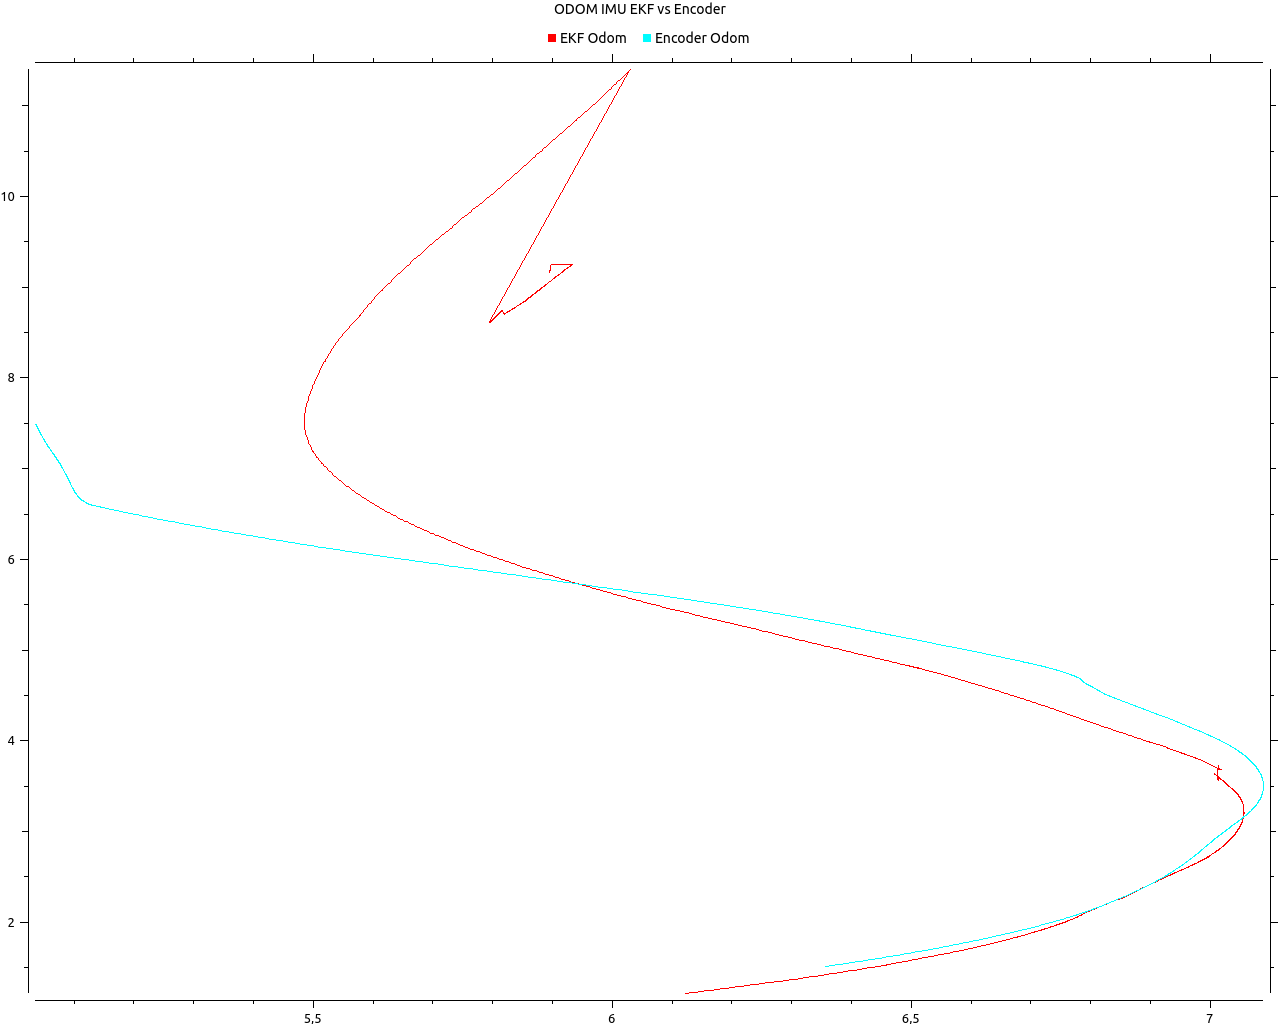
\includegraphics[width=\textwidth]{Pictures/odom pose comp}
	\caption{pose comparison wheel odom + IMU}
	\label{pose comparison wheel odom + IMU}

\end{figure}

\begin{figure}
	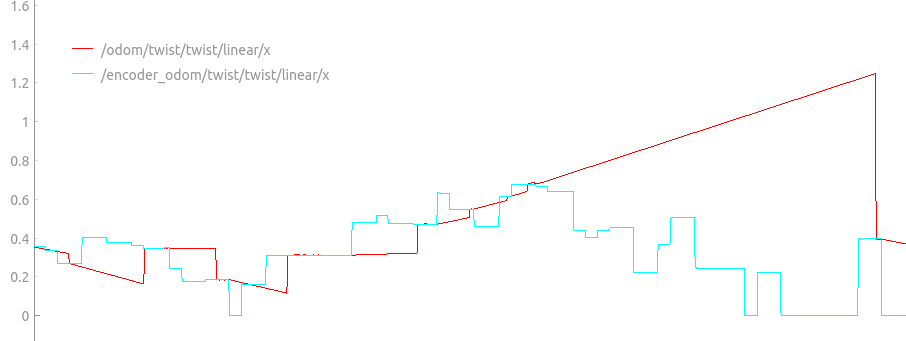
\includegraphics[width=\textwidth]{Pictures/comparison odom}
	\caption{velocity comparison wheel odom + IMU}
	\label{velocity comparison wheel odom + IMU}

\end{figure}


To fix this a logical approach is to include more data about the robots movement. Fortunately robot\_localization has an input for command velocities such as velocities produced by move base. While the command velocity does not provide any measurement in the real world the ekf filter can profit from knowing what the velocity actually should be.\\
It is very important to set the control timeout to a value that is larger than the cycle time of move\_base. Otherwise this will lead to translational offsets caused by too low estimate for the velocities like shown in Figure \ref{velwithcmd}.

\begin{figure}
	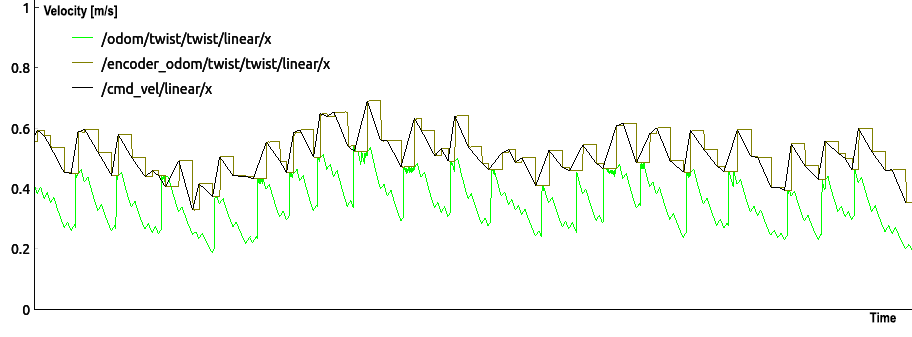
\includegraphics[width=\textwidth]{Pictures/velocity comp}
	\caption{velocity offset caused by too low control timout}
	\label{velocity offset}

\end{figure}


After the inclusion of the command velocity the acceleration limits in the configuration file of robot\_localization can be set equal to the limits in the local planner.

When observing both the pose and velocities again it is noticeable, that the odometry has drastically improved as pictured in Figure \ref{Odometry comparison wheel odomIMUcmdvel}, equally the velocities stay closer together as pictured in \ref{velwithcmd}.

\begin{figure}
	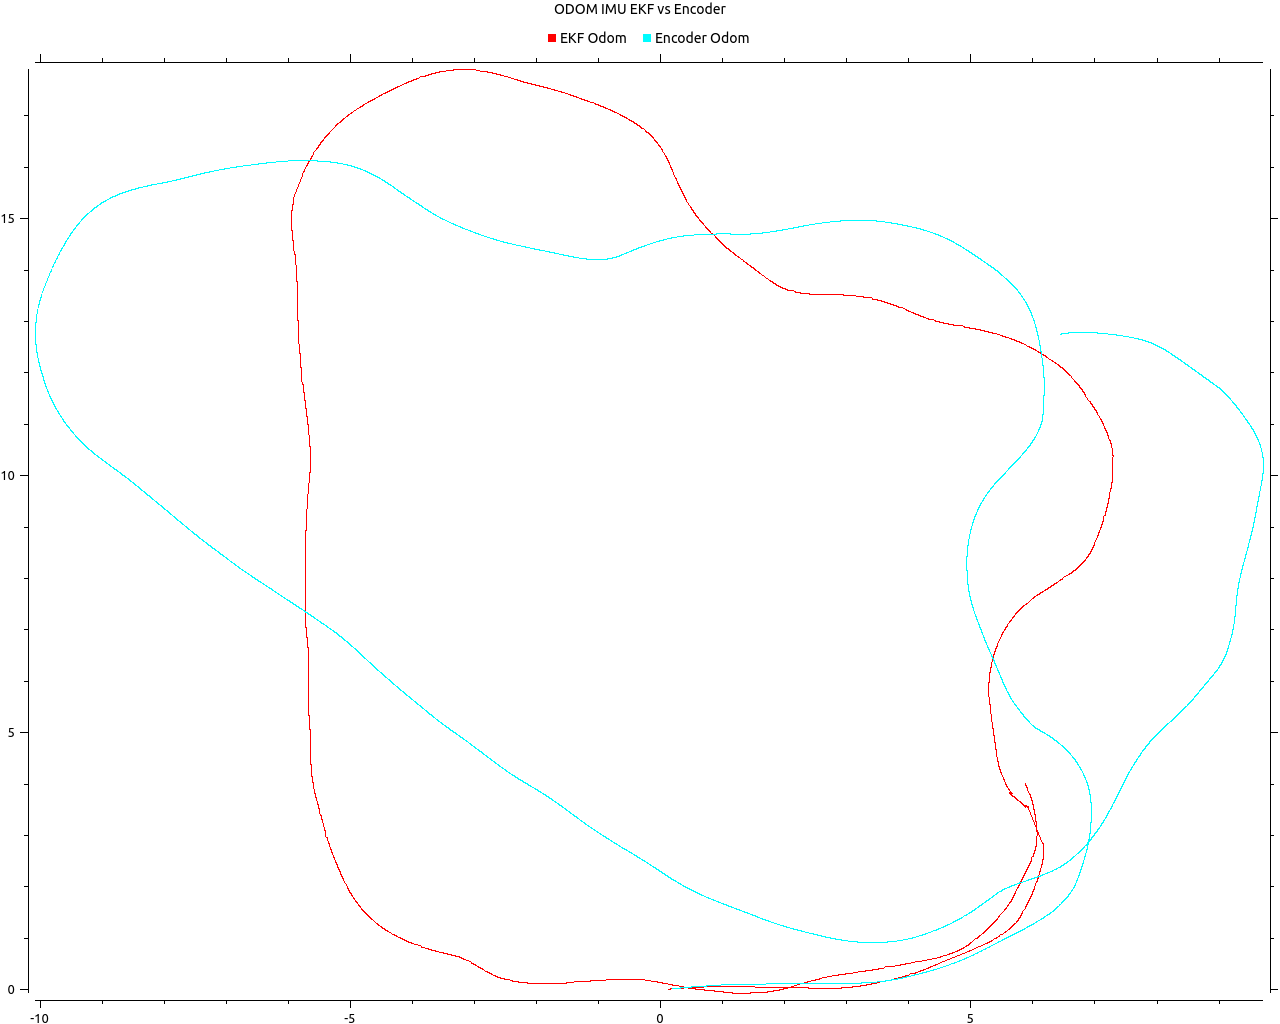
\includegraphics[width=\textwidth]{Pictures/odom after one round}
	\caption{Odometry comparison wheel odom + IMU + cmd\_vel}
	\label{Odometry comparison wheel odomIMUcmdvel}

\end{figure}
\begin{figure}
	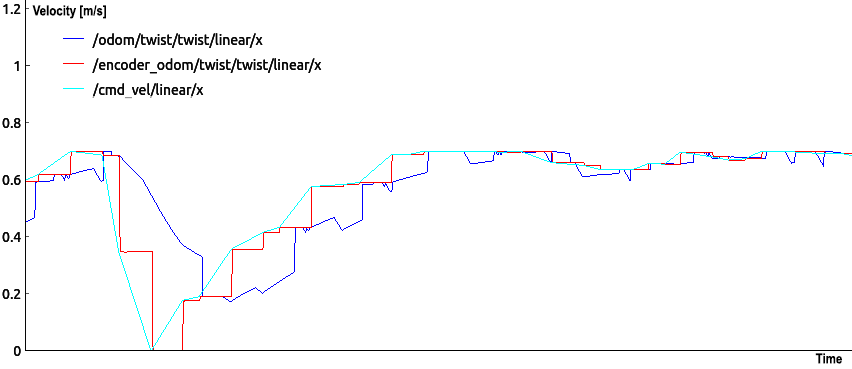
\includegraphics[width=\textwidth]{Pictures/circle vel}
	\caption{Velocity comparison with cmd\_vel}
	\label{velwithcmd}
\end{figure}



\begin{figure}
	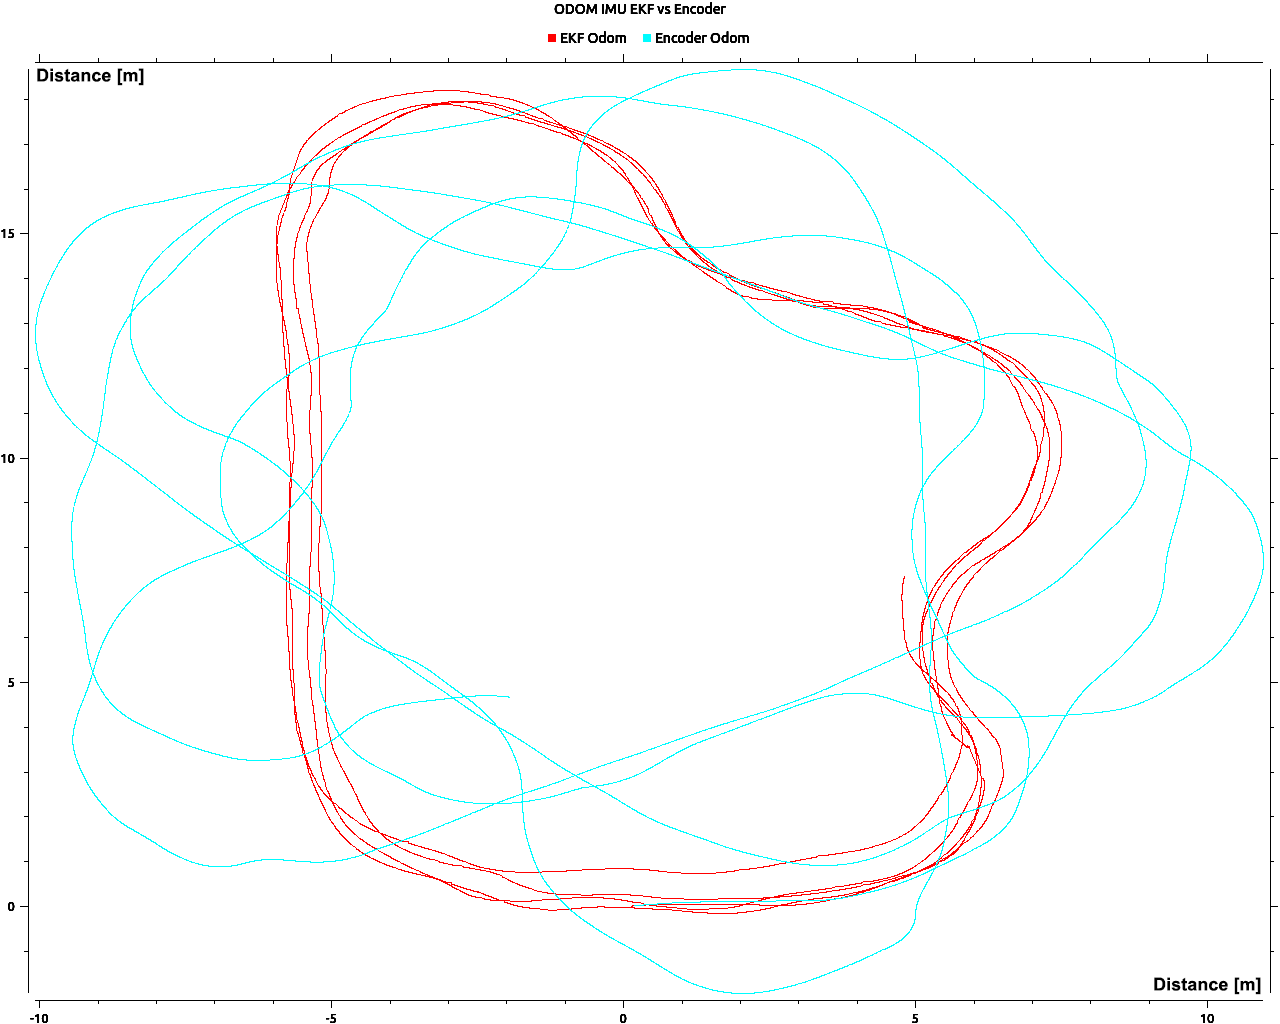
\includegraphics[width=\textwidth]{Pictures/odom comp multiple rounds}
	\caption{Odom comparison multiple rounds}
	\label{Odom comparison multiple rounds}

\end{figure}

Even after four rounds the odometry has not gained a large error in both translational and rotational as pictured in Figure \ref{Odom comparison multiple rounds}, furthermore the difference between the original odometry of the wheel encoders to the odometry from robot localization is quite remarkable.

After the rotantional and translational errors are marginal the scale of the odometry needs to be checked.
To isolate the different errors from the scaling error a circular track is build with a radius of 10 meter. Since the turning radius is constant this isolates the rotational error which can be seen at the graph of the wheel odometry in Figure \ref{circular track}.\\
The radius was chosen that high so potential errors are amplified and easier detectable.\\

Since the robot is driving on the lane and not on the middle road marking the expected radius is 10,45 meter. When evaluating the EKF odom in Figure \ref{circular track} we see that the scale is very precise.
 
\begin{figure}
	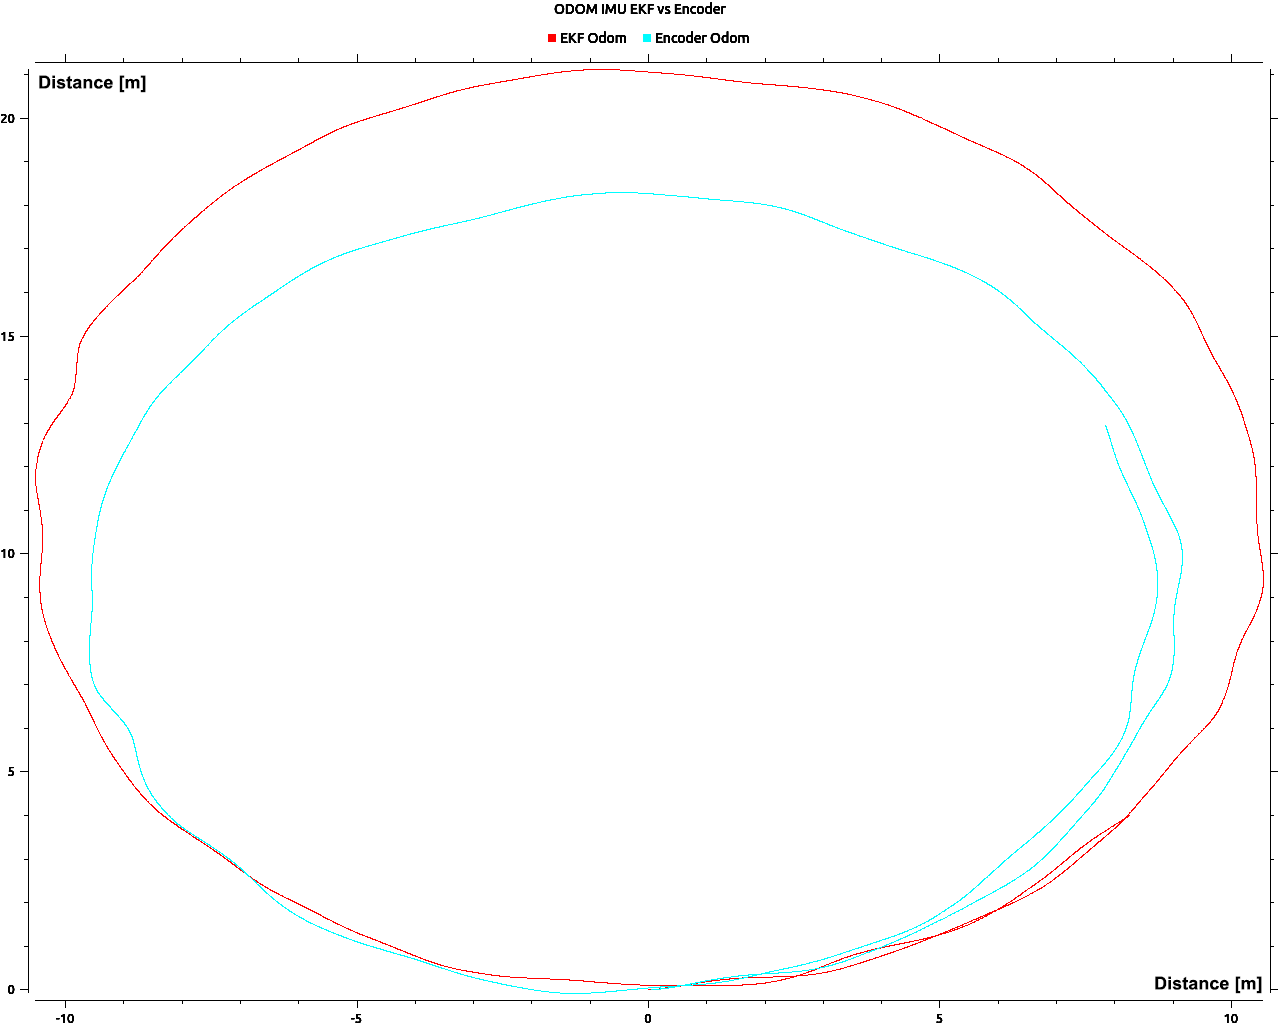
\includegraphics[width=\textwidth]{Pictures/circle odom}
	\caption{Odom comparison circular track}
	\label{circular track}

\end{figure}

As a final test the odometry from the robot\_localization node is compared to the true position from the simulation.

 \begin{figure}
	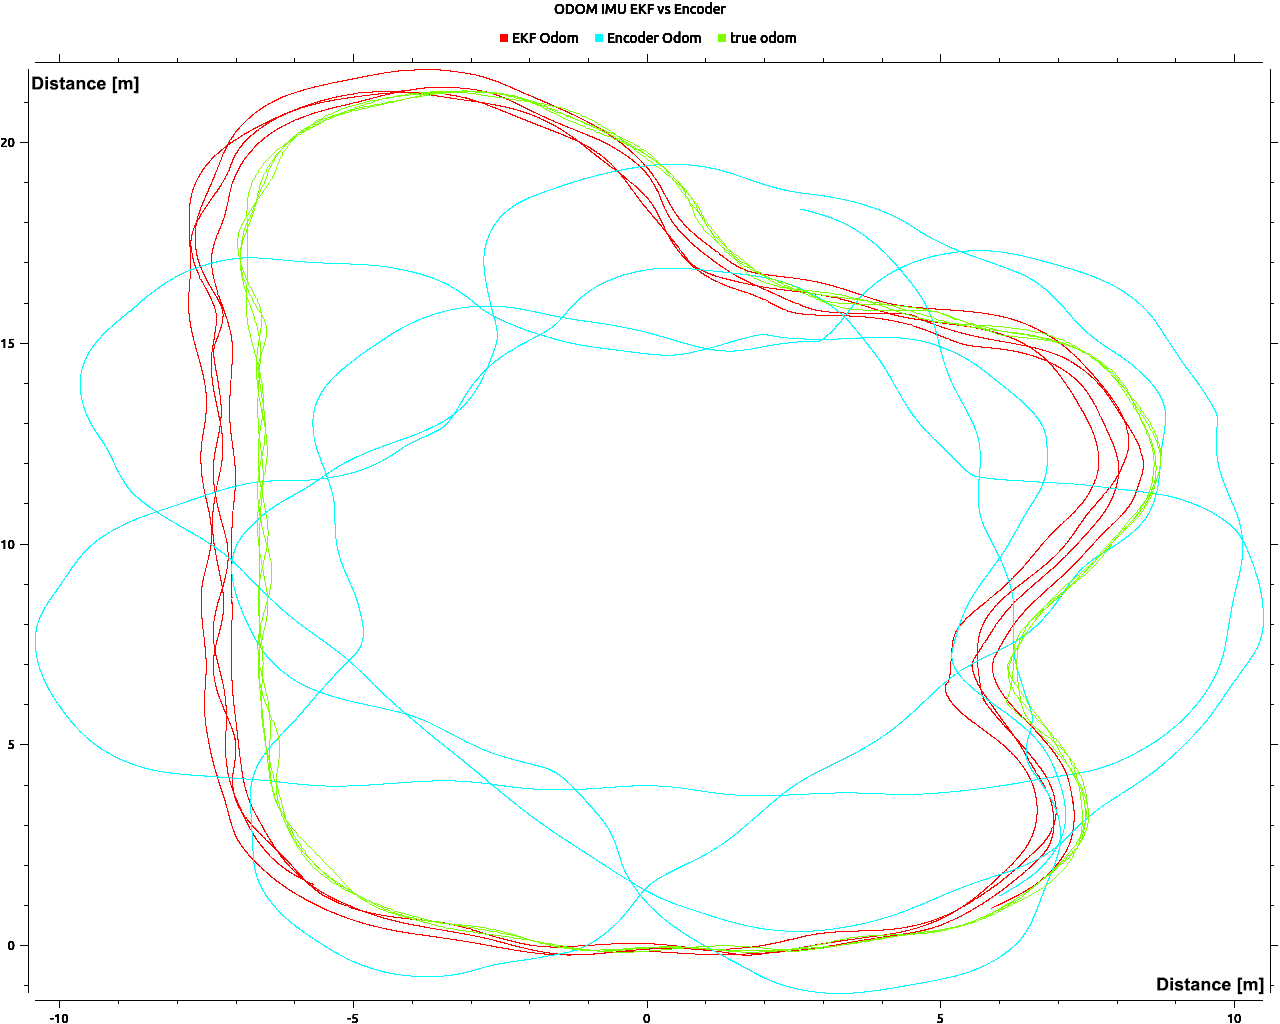
\includegraphics[width=\textwidth]{Pictures/odom with true}
	\caption{Comparison with true position}
	\label{trueodom}
\end{figure}

The comparison in Figure \ref{trueodom} shows, that the filtered odometry has a slight translational offset, but is very similar to the true odometry extracted from the simulation, hence it will be considered as sufficient for the navigation.


\section{Lidar test}


The Lidar sensor is simulated with realistic noise and errors. This also introduces the well known edge error in Laser distance measurement. 

When using a ``realistic'' lidar to project obstacles into the costmap this error produces a lot of lethal point like obstacles that significately hinder navigation as visible in Figure \ref{unfiltered lidar}.

\begin{figure}[H]
	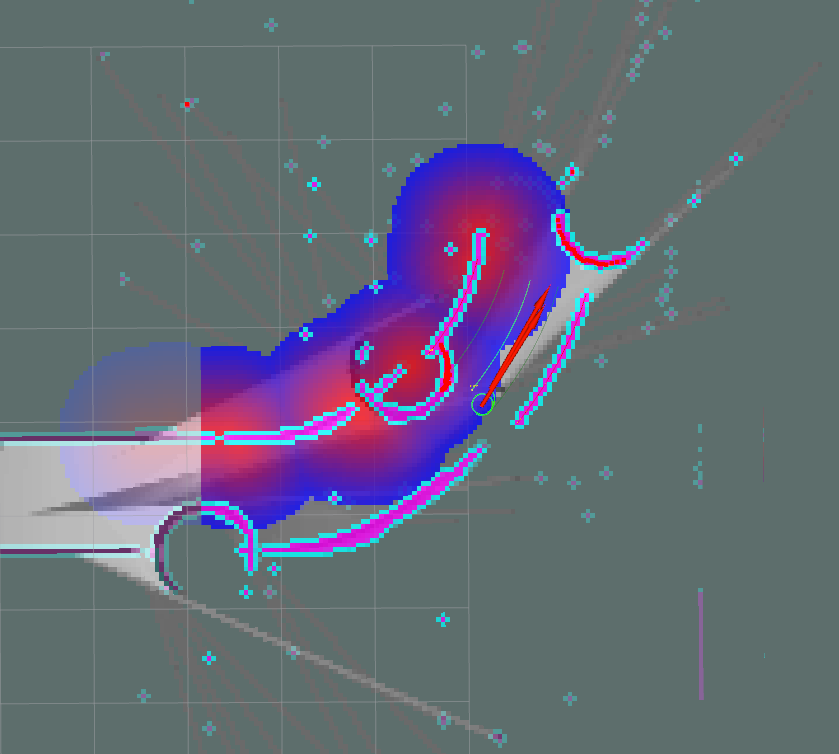
\includegraphics[width=\textwidth]{Pictures/Needs filtering of Laser}
	\caption{Lidar Test result}
	\label{unfiltered lidar}
\end{figure}

\subsection{Optimization}
To remove these error measurements the ROS package ``laser\_filters'' can be used. Among many different filter plugins that can be constructed into a filter chain it features the filter plugin ``ScanShadowFilter'' that is developed to remove the veiling effect around obstacles cause by the edge effect \cite{laserfilters}.


Figure \ref{lasercomp} shows a comparison between the filtered and not filtered laser scan, while keeping the data for 10 seconds. This allows to see the quickly jumping outliers caused by the edge effect. The filter seems well configured since the filtered points have no single outlier but still featuring a very good representation of the measured obstacle.

\begin{figure}[H]
	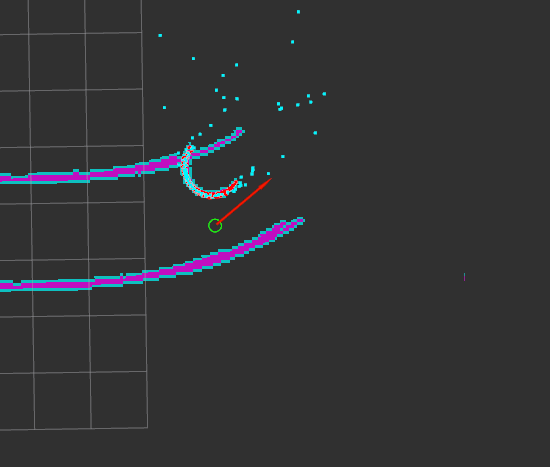
\includegraphics[width=\textwidth]{Pictures/LASERFILTER COMP}	
	\caption{comparison between filtered and not filtered laser scan (red - filtered, turquoise - raw)}
	\label{lasercomp}
\end{figure}

\section{road\_detection test}

As pictured in Figure \ref{longdurroad} the performance of the road detection converges to ca. 98.8\%. At the beginning the graph is not as reliable since there have not yet been enough measurements.\\

The duration of the test was roughly 1.5 hours of continuous navigation without obstacles in the simulation.

\begin{figure}[H]
	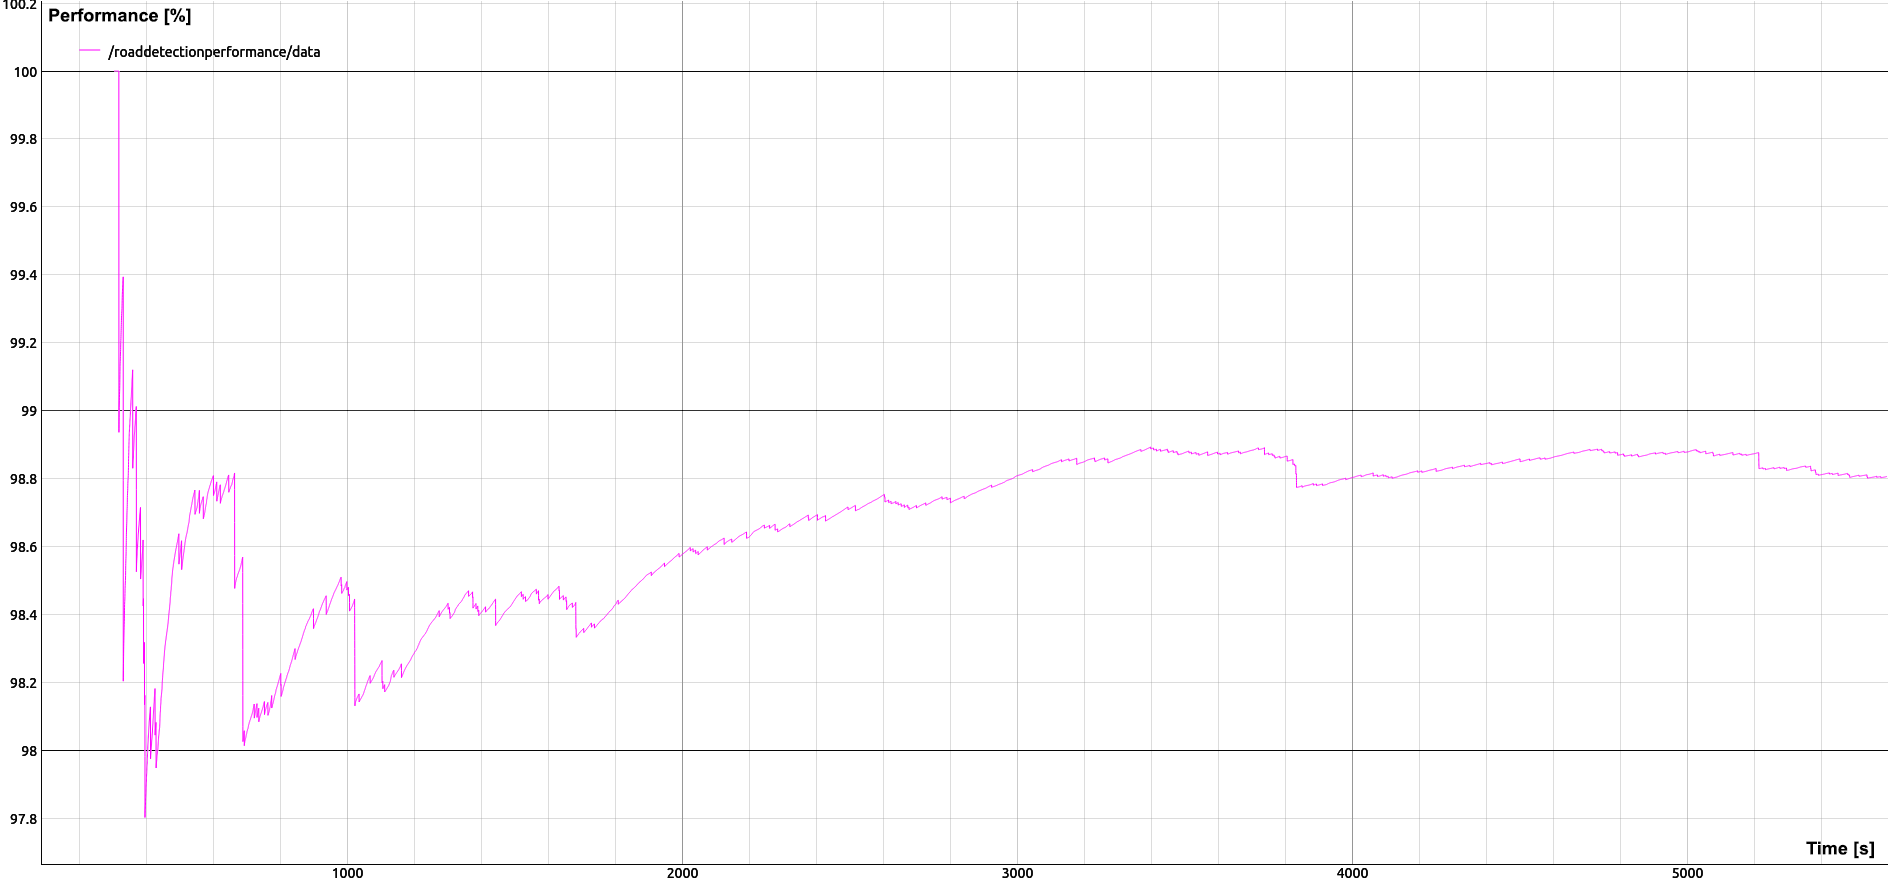
\includegraphics[width=\textwidth]{Pictures/long duration road detection test}
	\caption{roadRecordEvaluation during long duration test}
	\label{longdurroad}
\end{figure}





\section{complete system test}
The results of chapter \ref{configurationandtesting} will be discussed in the following part. The complete system test will be discussed first and afterwards the test of the subsystems\\

The results show that the navigation works really good, when no obstacle is on the road. The robot drives almost constantly on the right line and only rarely enters the left lane. These rare scenarios are mostly caused by the bug in the global\_planner mentioned in section \ref{globalplannertest}.\\

With obstacles on the left lane the navigation still works reasonably well, but sometimes the robot transitions directly after passing an obstacle, since the left lane has not been detected behind the obstacle and therefore has not been inflated. Therefore the global planner pushes the robot to the left.\\

Finally when obstacles are on the right lane the robot manages to avoid most of them. But after reentering the right lane the navigation sometimes has a small oscillation along the middle road marking as visible in Figure \ref{rightobsfinal}. Also observable where cases, where the robot left the road during remerging on the right lane since the prediction of the PoseFinder was to inaccurate and the road was not detected again after starting the avoidance.\\

This 





